
In this section, we propose a unified computational account of \emph{ad hoc} coordination and convention formation that aims to address these three empirical puzzles. 
We begin from first principles: What is the core computational problem that must be solved to achieve successful communication?
Classically, this problem has been formulated in terms of coding and compression \cite{Shannon48}. 
An intended meaning in the speaker's mind must be encoded as a signal that is recoverable by the receiver after passing through a noisy transmission channel.
This transmission problem has since been enriched to account for \emph{pragmatics} -- the ability of speakers and listeners to use context and social knowledge to go beyond the literal meaning of messages \cite{RosenbergCohen66_ReferentialProcesses,sperber1986relevance}.
We take the Rational Speech Act framework \cite<RSA;>{FrankGoodman12_PragmaticReasoningLanguageGames,goodman_pragmatic_2016,FrankeJager16_ProbabilisticPragmatics} as representative of this current synthesis, formalizing communication as recursive social inference in a probabilistic model (see Appendix A for technical details.)
In the next section, we review this basic framework and raise two fundamental computational problems facing it.
These problems motivate the introduction of continual learning in the CHAI model.

\subsection{Models of communication with static meaning}

For concreteness, we restrict our scope to reference in a context $\mathcal{C}$ containing a discrete set of objects $o\in\mathcal{O}$, but the same formulation aims to apply more generally.
In this referential setting, the RSA framework defines a pragmatic speaker, denoted by $S_1$, who must choose an utterance $u$ that will allow their partner to choose a particular target object $o^* \in \mathcal{C}$.
They attempt to satisfy Gricean Maxims \cite{Grice75_LogicConversation} by selecting utterances according to a utility function $U(u;o)$ that balances informativity to an imagined listener against the cost of producing an utterance.
Specifically, $S_1$ chooses from a ``softmax distribution'' concentrating mass on the utterance that maximizes $U(u;o)$ to an extent modulated by a free parameter $\alpha_S \in[0,\infty]$:
\begin{align}
S_1(u | o) & \propto   \exp\{\alpha_S \cdot U(u; o)\}
\end{align}
For $\alpha_S = 1$, this decision rule corresponds to Luce's choice axiom \cite{luce1959individual}. 
Larger settings of $\alpha_S$ concentrate more probability on the single utterance maximizing utility.

The basic speaker utility function in the RSA framework is defined as follows:
\begin{align}
U(u; o) & = (1-w_C) \cdot \underbrace{\log L_0(o | u)}_{\mathclap{\text{informativity}}} -\, w_C \cdot \underbrace{c(u)}_{\mathclap{\text{cost}}} \label{eq:RSAspeaker}
\end{align}
where $c(u)$ is a function giving the cost of producing $u$, assuming longer utterances are more costly, and $w_C \in [0,1]$ is a second free parameter controlling the relative weight of informativity and parsimony in the speaker's production.
Critically, the informativity term in Eq.~\ref{eq:RSAspeaker} is defined by how well $u$ transmits the intended target $o^*$ to an imagined listener.
The simplest imagined listener, $L_0$, is typically called the ``literal listener'' because they are assumed to identify the target relying only on the literal meaning of the received utterance, without appealing to further social reasoning about the speaker.
That is, the probability of the imagined listener choosing object $o$ is simply assumed to be proportional to the meaning of $u$ under some (static) lexical function $\mathcal{L}$:
\begin{align}
L_0(o | u) &\propto  \mathcal{L}(u,o)\nonumber
\end{align}
Throughout this paper, we will take $\mathcal{L}$ to be a traditional Boolean function evaluating whether or not the expression $u$ applies to the entity in question\footnote{Due to the current limitations of representing lexical meaning in formal semantics, it has not been straightforward to specify a truth-conditional function explaining listener behavior for natural-language utterances (e.g. what makes one drawing belong in the literal extension of ``upside-down martini glass'' but not another, when neither of them are literally martini glasses?) This representation is convenient for our simulations, where we consider all possible discrete mappings between utterances and objects in the context, but better representations of lexical meaning may be substituted \cite<see>{potts2019case}. For example, Appendix B works out an example using a real-valued, continuous function \cite{degen2020redundancy} such as those learned by multi-modal neural networks \cite{monroe_colors_2017,achlioptas2019shapeglot,hawkins2019continual}.}:
$$
\mathcal{L}(u,o) = \left\{ \begin{array} {rl} 1 & \textrm{if $o \in \den{u}$} \\ 0 & \textrm{otherwise} \end{array}\right.
$$

%Finally, we may then define a pragmatic listener $L_1$ that inverts their own internal model of an imagined speaker, inferring which intended referent $o\in\mathcal{C}$ would best explain the speaker's choice of utterance $u$:
%\begin{align}
%L_1(o | u) \propto   \exp\{w_L \cdot \log S_1(u | o)\}\nonumber
%\end{align}
%Intuitively, this listener is able to account for alternative utterances the speaker could have chosen to produce.
%For example, if an alternative utterance $u'$ would have perfectly referred to some object $o$, then the fact that the speaker did \emph{not} choose to say $u'$ suggests $o$ is not the intended referent. 

\subsection{Two fundamental problems for static meaning}

The RSA framework and its extensions provide an account for a variety of important phenomena in pragmatic language use \cite<e.g.>{Scontras_problang,KaoWuBergenGoodman14_NonliteralNumberWords,TesslerGoodman16_Generics,LassiterGoodman15_AdjectivalVagueness}.
Yet it retains a key assumption from classical models: that the speaker and listener must share the same literal ``protocol'' $\mathcal{L}$ for encoding and decoding messages.
In this section, we highlight two under-appreciated challenges of communication that complicate this assumption. 

The first problem arises from the existence of \emph{variability} throughout a language community \cite{kidd2018individual,wangidiosyncratic}. 
Different listeners may recover systematically different meanings from the same message, and different speakers may express the same message in different ways.
For example, doctors may fluently communicate with one another about medical conditions using specialized terminology that is meaningless to patients. 
The words may not be in the patient's lexicon, or common words may be used in non-standard ways.
That is, being fluent speakers of the same language does not ensure agreement for the relevant meanings expressed in every context. 
Different partners may be using different functions $\mathcal{L}$.

The second problem arises from the \emph{non-stationarity} of the world. 
Agents are continually presented with new thoughts, feelings, and entities, which they may not already have efficient conventions to talk about \cite{gerrig1988beyond}.
For example, when new technology is developed, the community of developers and early adopters must find ways of referring to the new concepts they are working on (e.g. \emph{tweeting}, \emph{the cloud}). 
Or, when researchers design a new experiment with multiple conditions, they must find ways of talking about their own \emph{ad hoc} abstractions, often converging on idiosyncratic names that can be used seamlessly in meetings.
That is, any fixed $\mathcal{L}$ shared by a group of speakers at one moment in time can quickly become outdated \cite<see>[for a demonstration of the related problems posed by non-stationary for large neural language models]{lazaridou2021pitfalls}.
We must have some ability to extend our language on the fly as needed.

\subsection{CHAI: A model of dynamic meaning}

Rather than assuming a monolithic, universally shared language, we argue that agents solve the fundamental problems posed by variability and non-stationarity by attempting to continually, adaptively \emph{infer} the system of meaning used by their current partner.
When all agents are continually learning in this way, and changing their own behavior to best respond, we will show that they are not only able to coordinate on local, \emph{ad hoc} meanings or pacts with specific partners but also abstract away \emph{conventions} that are expected to be shared across an entire community.
We introduce the CHAI (Continual Hierarchical Adaptation through Inference) model in three steps, corresponding to how it formalizes the three core capacities \textbf{C1-C3}: hierarchical uncertainty about meaning, online partner-specific learning, and inductive generalization.

\paragraph{C1:~Representing variability in meaning via structured uncertainty} 

When an agent encounters a communication partner, they must call upon some representation about what they expect different signals will mean to that partner. 
We therefore replace the monolithic, static function $\mathcal{L}$ with a \emph{parameterized family} of lexical meaning functions by $\mathcal{L}_{\phi}$, where different values of $\phi$ yield different possible systems of meaning. 
To expose the dependence on a fixed system of meaning, Eq.~\ref{eq:RSAspeaker} can be re-written to give behavior under a fixed value of $\phi$:
\begin{align}
L_0(o | u, \phi) &\propto  \mathcal{L}_\phi(u,o)\hfill\label{eq:RSA} \\
U(u; o, \phi) & = (1-w_C) \cdot \log L_0(o | u, \phi) -\, w_C \cdot c(u) \nonumber  \\
S_1(u | o,\phi) & \propto   \exp\{\alpha_S \cdot U(u; o, \phi)\} \nonumber 
%L_1(o | u,\phi) & \propto   \exp\{w_L \cdot \log S_1(u | o, \phi) \nonumber \}
\end{align}

While we will remain agnostic for now to the exact functional form of $\mathcal{L}_\phi$ and the exact parameter space of $\phi$, there are two computational desiderata we emphasize.
First, given the challenge of variability raised in the previous section, these expectations ought to be \emph{sensitive to the overall statistics of the population}. 
That is, an agent should know that more people will share the meaning of some words than others, and should conversely expect more consensus about how to refer to some concepts than others.
Second, expectations about which meanings will be evoked for a given utterance and which utterances are expected to be used to express a meaning should be \emph{sensitive to the social identity of one's partner}.%: a cardiologist should have different expectations about a long-time colleague than a new patient.

The first desideratum -- the ability to represent variability in the population -- motivates a \emph{probabilistic} formulation.
Instead of holding a single static function $\mathcal{L}_{\phi}$, which an agent assumes is shared perfectly in common ground (i.e. one $\phi$ for the whole population), we assume each agent maintains uncertainty over the exact meaning of each word as used by different partners.
In a Bayesian framework, this uncertainty is specified by a prior probability distribution $P(\phi)$ over possible function parameters.
For example, imagine a doctor giving a diagnosis to a new patient.
Under some possible values of $\phi$, a piece of medical jargon like ``sclerotic aorta'' refers unambiguously to the patient's heart condition.
Under other values of $\phi$, it has a less clear meaning. 
A doctor with good bedside manner should assign some probability to each possibility rather than assuming everyone will share the same precise meaning they learned in medical school. 
Importantly, this variability will be different for different words: likely more people share the meaning of ``dog'' than ``sclerotic aorta''.
This core idea of introducing uncertainty over a partner's lexical semantics has previously been explored in the context of one-shot pragmatic reasoning, where it was termed \emph{lexical uncertainty} \cite{BergenGoodmanLevy12_Alternatives,PottsLevy15_Or,bergen_pragmatic_2016,potts2016embedded}, as well as in the context of iterated dyadic interactions \cite{SmithGoodmanFrank13_RecursivePragmaticReasoningNIPS}. 

\begin{figure}[b!]
\centering
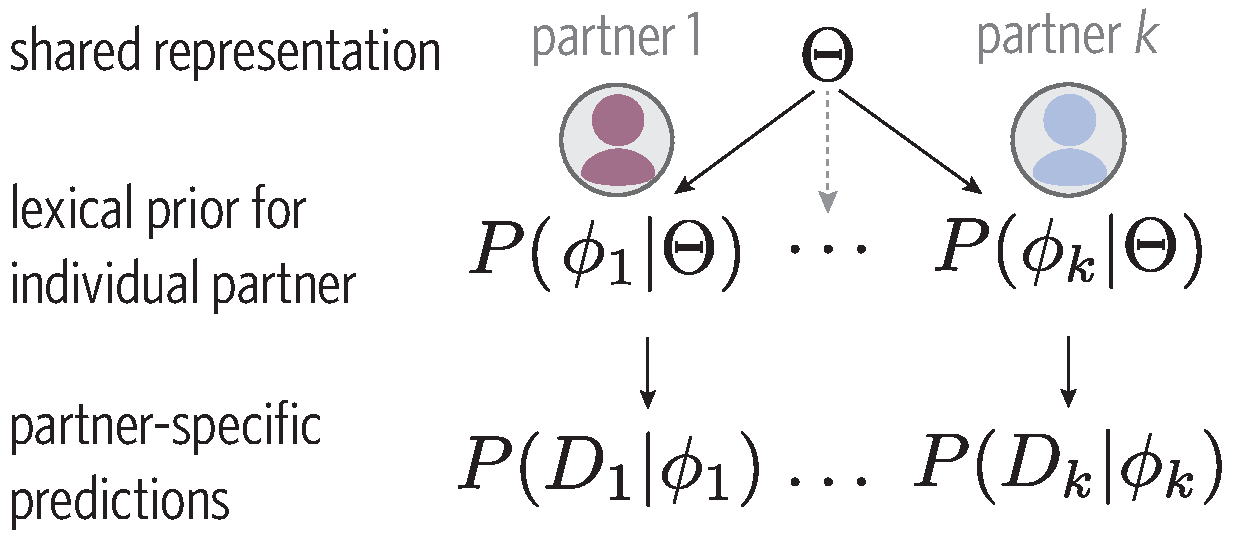
\includegraphics[scale=0.35]{./figures/task1_model.pdf}
\vspace{.5em}
\caption{\emph{Schematic of hierarchical model.} At the highest level, denoted by $\Theta$, is a representation of aspects of meanings expected to be shared across all partners. These conventions serve as a prior for the systems of meanings used by specific partners, $\phi_k$. Partner-specific representations give rise in turn to predictions about language use $P(D_k|\phi_k)$, where $D_k$ represents observations in a communicative interaction with partner $k$. By inverting this modeld, agents can adapt to \emph{local, ad hoc} conventions and gradually update their beliefs about conventions in their broader community.}
\label{fig:model_schematic}
\end{figure}

Second, this representation should also, in principle, be sensitive to the social identity of the partner: a doctor should be able to form different expectations about a new colleague than a new patient \cite{clark_communal_1998}.
This desideratum -- sensitivity to partner-specific meanings -- motivates a \emph{hierarchical} model, where uncertainty is represented by a multi-level prior. 
At the highest level of the hierarchy is \emph{community-level} uncertainty $P(\Theta)$, where $\Theta$ represents an abstract ``overhypothesis'' about the overall distribution of all possible partners. 
This level can be viewed as a representation of long-term ``communal lexicons'' about common knowledge based on community membership \cite{ClarkMarshall1981}. 
$\Theta$ then parameterizes the agent's \emph{partner-specific} uncertainty $P(\phi_{k} | \Theta)$, where $\phi_k$ represents the specific system of meaning used by partner $k$ (see Fig.~\ref{fig:model_schematic}). 
$\phi_k$ can be viewed as the ``idiolect'' that has been fine-tuned to account for partner-specific common ground and conceptual pacts from previous interactions\footnote{We focus for simplicity on this basic two-layer hierarchy, but the model can be straightforwardly extended to representing uncertainty at intermediate layers of social structure, including whether partners belong to distinct sub-communities \cite<e.g. represented by discrete latent variables>{GershmanEtAl17_StructureSocialInfluence,gershman2020social}, which may explain code-switching \cite{auer_code-switching_2013,hawkinsrespect} and other social inferences based on language use \cite{kinzler2021language,IsaacsClark87_ReferencesExpertsNovices,roberts_experimental_2010}.}.

To integrate lexical uncertainty into our speaker and listener models, we assume they each act in a way that is expected to be successful \emph{on average}, under likely values of $\phi_k$ \cite{SmithGoodmanFrank13_RecursivePragmaticReasoningNIPS}.
In other words, they sample actions by marginalizing over their own beliefs $P_S(\phi_k)$ or $P_L(\phi_k)$ about different meanings their partner $k$ may be using.
\begin{align}
L(o|u) &\propto   \exp\left\{\alpha_L\cdot \textstyle{\int} P_L(\phi_k)  \log S_1(u|o, \phi_k)\,\,d\phi_k\right\}\nonumber\\
S(u|o) &\propto  \exp\left\{\alpha_S \cdot \textstyle{\int} P_S(\phi_k)  U(u; o, \phi_k) \,\,d\phi_k\right\}\label{eq:marginalized}
\end{align}
where $\alpha_S, \alpha_L \in[0,\infty]$ control the speaker's and listener's soft-max optimality, respectively\footnote{We denote $L$ and $S$ without a subscript because they are the only speaker and listener models we use in simulations throughout the paper -- the subscripted definitions are internal constructs used to define these models -- but in the terminology of the RSA framework they represent $L_1$- and $S_1$-level pragmatic agents with lexical uncertainty. We found that higher levels of recursion were not  necessary to derive the phenomena of interest, but $L_n$ and $S_n$-level lexical uncertainty models may be generalized by replacing $S_1$ in the listener equation, and $L_0$ in the speaker's utility definition, with standard RSA definitions of $n-1$-level agents \cite<see also>{zaslavsky2020rate}.}.

\paragraph{C2: Online learning via partner-specific inference}

The formulation in Eq.~\ref{eq:marginalized} derives how agents ought to act under uncertainty about the lexicon being used by their partner, $P(\phi_k)$.
But how do beliefs about their partner change over time?
Although an agent may begin with significant uncertainty about the system of meaning their partner is using in the current context, further interactions provide useful information for reducing that uncertainty and therefore improving the success of communication.
In other words, \emph{ad hoc} convention formation may be re-cast as an inference problem.
Given observations $D_k$ from interactions with partner $k$, an agent can update their beliefs about their partner's latent system of meaning following Bayes rule:
\begin{equation}
\begin{array}{rcl}
\label{eq:joint_inference}
P(\phi_k, \Theta | D_k)  & \propto &  P(D_k | \phi_k, \Theta) P(\phi_k, \Theta) \\
                           & =   & P(D_k | \phi_k) P(\phi_k | \Theta) P(\Theta)
\end{array}
\end{equation}
This joint inference decomposes the partner-specific learning problem into two terms, a prior term $P(\phi_k | \Theta)P(\Theta)$ and a likelihood term $P(D_k | \phi_k)$.
The prior term captures the idea that, in the absence of strong evidence of partner-specific language use, the agent ought to regularize toward their background knowledge of conventions: the aspects of meaning that all partners are expected to share in common.
The likelihood term represents predictions about how a partner would use language in context under different underlying systems of meaning.

Importantly, the posterior obtained in Eq.~\ref{eq:joint_inference} allows agents to explicitly maintain \emph{partner-specific expectations}, as used in Eq.~\ref{eq:marginalized}, by marginalizing over community-level uncertainty:
\begin{equation}
P(\phi_k | D_k) =  \int_{\Theta}P(\phi_k, \Theta | D_k)  d\Theta
\end{equation}
We will show that when agents learn about their partner in this way, and adjust their own production or comprehension accordingly (i.e.~Eq.~\ref{eq:marginalized}), they are able to coordinate on stable \emph{ad hoc} conventions.

\paragraph{C3: Generalization to new partners via hierarchical induction}

The posterior in Eq.~\ref{eq:joint_inference} also provides an inductive pathway for partner-specific data to inform beliefs about community-wide conventions.
Agents update their beliefs about $\Theta$, using data accumulated from different partners, by marginalizing over beliefs about specific partners:
\begin{equation}
\begin{split}
    P(\Theta | D)  = & \int_{\phi} P(\phi, \Theta | D) d\phi \\
%                     \propto & P(\Theta) \int_{\phi} P(D_k | \phi_k) P(\phi_k | \Theta) d\phi
\end{split}
\end{equation}
where $D = \bigcup_{k=1}^N D_k$, $\phi = \phi_1 \times \dots \times \phi_N$, and $N$ is the number of partners previously encountered. 
Intuitively, when multiple partners are inferred to use similar systems of meaning, beliefs about $\Theta$ shift to represent this abstracted knowledge: it becomes more likely that novel partners in one's community will share it as well.
Note that this population-level posterior over $\Theta$ not only represents what the agent has learned about the central tendency of the group's conventions, but also the \emph{spread} or variability, capturing the notion that some word meanings may be more widespread than others.

The updated $\Theta$ should be used to guide the prior expectations an agent brings into a subsequent interactions with strangers.
This transfer is sometimes referred to as ``sharing of strength'' or ``partial pooling'' because pooled data is smoothly integrated with domain-specific knowledge.
This property has been key to explaining how the human mind solves a range of other difficult inductive problems in the domains of concept learning \cite{KempPerforsTenenbaum07_HBM, tenenbaum_how_2011}, causal learning \cite{KempPerforsTenenbaum07_HBM,KempGoodmanTenenbaum10_LearningToLearn},  motor control \cite{berniker2008estimating}, and speech perception \cite{kleinschmidt2015robust}.
One consequence is the ``blessing of abstraction,'' \cite{GoodmanUllmanTenenbaum11_TheoryOfCausality} where it is possible under certain conditions for beliefs about the community's conventions \emph{in general} to outpace beliefs about the idiosyncracies of individual partners \cite{gershman2017blessing}.

\subsection{Further challenges for convention formation}

The formulation in the previous section presents the core of CHAI.
Here, we highlight several additional features addressing more specific challenges raised by prior work on communication and which we will encounter in the simulations reported in the remainder of the paper. 
Our organization of these details is motivated by the analysis of \citeA{spike_minimal_2017}, who highlighted three common issues that all accounts of convention formation must address: (1) the form of feedback available, (2) the influence of memory and temporal discounting, and (3) the form of pragmatic reasoning being used.
Finally, we set up the basic simulation framework that will be used throughout the rest of the paper.

\paragraph{The role of social observation}

Learning and adaptation depend critically on the availability and quality of social observations $D_k$ (Eq.~\ref{eq:joint_inference}).
If the speaker has no way of probing the listener's understanding, or if the listener has no way of comparing their interpretation against the speaker's intentions, however indirectly, they can only continue to rely on their prior expectations, with no ground for conventions to form  \cite{HupetChantraine92_CollaborationOrRepitition,GarrodFayLeeOberlanderMacLeod07_GraphicalSymbolSystems}.
Communication is empirically hindered under degraded observation conditions  \cite{KraussWeinheimer66_Tangrams,KraussBricker67_Delay,KraussEtAl77_AudioVisualBackChannel,SchoberClark89_Overhearers}, and we have all been in situations where we thought we were on the same page with a partner and only realized that we misunderstood much later, when the consequences because clear.
In principle, we expect that $D_k$ should reflect all relevant sources of information that may expose an agent's state of understanding or misunderstanding.
Not just ostensive signals like pointing \cite{vandeBraak2021}, but verbal and non-verbal backchannels (e.g. \emph{mmhmm}, nods or quizzical looks), forms of self-initiated and other-initiated repair \cite<e.g. clarification questions or requests for confirmation>{SchegloffEtAl77_Repair, DingemanseEtAl15_RepairUniversal,arkel2020simple}, and downstream actions taken in the world (e.g. attempts to follow instructions).

While incorporating these richer sources of information presents an exciting line of future work, we restrict our scope to the feedback traditionally provided by the empirical repeated reference task, where the speaker's intended target and the listener's response are revealed at the end of each trial. 
Formally, this information can be written as a set of tuples $D_k = \{o^*, u', o'\}_{t=1}^T$, where $o^*$ denotes the speaker's intended target, $u'$ denotes the utterance they produced, and $o'$ denotes the listener's response, on each previous trial $t$.
To specify the likelihoods in Eq.~\ref{eq:joint_inference} for this referential setting, we assume each agent should infer their partner's lexicon $\phi_k$ by conditioning on their \emph{partner's} previous behavior.
The listener on a given trial should use the probability that a speaker would produce $u$ to refer to the target $o^*$ under different $\phi_k$, i.e. $P_L(\{o^*, u', o'\}_t\, | \, \phi_k) = S_1(u'_t \,|\, o^*_t, \phi_k)$, and the speaker should likewise use the probability that their partner would produce response $o'$ after hearing utterance $u$, $P_S(\{o^*, u', o'\}_t \,|\, \phi_k) = L_0(o'_t \,|\, u'_t)$,

This symmetry, where each agent is attempting to learn from the other's behavior, creates a clear coordination problem\footnote{In some settings, agents in one role may be expected to take on more of the burden of adaptation, leading to an asymmetric division of labor \cite<e.g.>{MorenoBaggio14_AsymmetrySignaling}. This may be especially relevant in the presence of asymmetries in power, status, or capability \cite{MisyakEtAl14_UnwrittenRules}, but we leave consideration of such asymmetries for future work.}.
In the case of an error, where the agent in the listener role hears the utterance $u'$ and chooses an object $o'$ other than the intended target $o^*$, they will receive feedback about the intended target and subsequently condition on the fact that the speaker chose $u'$ to convey that target.
Meanwhile, the agent in the speaker role will subsequently condition on the likelihood that the listener chose the object $o'$ upon hearing their utterance.
In other words, each agent will subsequently condition on slightly different data leading to conflicting beliefs.
Whether or not agents are able to resolve early misunderstandings through further interaction and eventually reach consensus depends on a number of factors.

\paragraph{The role of memory and recency}

One important constraint is imposed by the basic cognitive mechanisms of memory.
It is unrealistic to expect that memory traces of every past interaction in the set of observations $D$ is equally accessible to the agent.
Furthermore, this may be to the agent's advantage.
Without a mechanism by which errors become less accessible, early misunderstandings may interfere with coordination much later in an interaction. 
One possible solution is to privilege more recent outcomes. 
Especially if a partner is assumed to change over time, then older data may provide less reliable cues to their current behavior.
Recency is typically incorporated into Bayesian models with a simple decay term in the likelihood function \cite{anderson2000adaptive,angela2009sequential,fudenberg2014recency,kalm2018visual}.
$$P(D_k | \phi_k) = \prod_{\tau=0}^T \beta^{\tau} P(\{o^*,u',o'\}_{T-\tau}\, |\, \phi_k)$$
where $\tau=0$ indexes the most recent trial $T$ and decay increases further back through time.
This decay term is motivated by the empirical power function of forgetting \cite{wixted1991form}, and can be derived by simply extending our hierarchical model down an additional layer \emph{within} each partner to allow for the possibility that they are using slightly different lexicons at different points in time; assuming a degree of auto-correlation between neighboring time points yields this form of discounting\footnote{While this simple decay model is sufficient for our reference games, it is clearly missing important mechanistic distinctions between working memory and long-term memory; for example, explaining convention formation over longer timescales may require an explicit model of consolidation or source memory. It is also consistent with multiple algorithmic-level mechanisms; for example, decay can be viewed as a form of weighted importance sampling, where more recent observations are preferentially sampled \cite{pearl2010online}, or a process where observations have some probability of dropping out of memory at each time step.}.


\paragraph{The role of pragmatics}

While natural languages are rife with ambiguous and polysemous terms, speaker and listeners must somehow resolve these ambiguities to be understood in context \cite{PiantadosiTilyGibson12_Ambiguity}\footnote{Indeed, \citeA{brochhagen2020signalling} has suggested that high degrees of lexical ambiguity and polysemy, i.e. high degrees of uncertainty over $\Theta$ in CHAI, are useful precisely because they allow much-needed flexibility supporting partner-specific adaptation.}. 
For example, \citeA{BrennanClark96_ConceptualPactsConversation} placed participants in a context where the target object $o^*$ was easily distinguished from other objects in the context $\mathcal{C}$ by a referring expression like $u=$``the shoe.''
In a second phase of the study, the context $\mathcal{C}'$ was switched to be a set of other shoes.
Even though there was strong precedent for referring to $o^*$ as ``the shoe,'' this description was no longer \emph{informative}: the speaker recognized that $u$ could apply equally well to all $o\in\mathcal{C}$ leading to potential ambiguity about which shoe they were referring to.
As a result, the speaker switched to a more specific utterance like $u'=$``the pennyloafer'' which unambiguously applied to $o^*$ in the new context.
In a third and final phase, the context reverted back to the original one, $\mathcal{C}$, but many speakers continued to use the more specific utterance $u'$ even though $u$ would have sufficed.
This example emphasizes how \emph{ad hoc} conventions or pacts may be sensitive to the context in which they form.

CHAI solves this problem by the principles of \textit{pragmatic reasoning} naturally instantiated in the RSA framework \cite{FrankGoodman12_PragmaticReasoningLanguageGames}, which plays two distinct roles.
First, our Gricean agents'  production and comprehension is guided by cooperative principles (Eq.~\ref{eq:marginalized}).
They do not only make passive inferences from observation, they participate in the interaction by \emph{using language} themselves.
Second, our agents assume that their \emph{partner} is also using language in a cooperative manner, which strengthens the inferences they may make about the underlying system of meanings their partner is using.
That is, we use the RSA equations as the linking function in the likelihood $P(D_k | \phi_k)$, representing an agent's prediction about how a partner with meaning function $\phi_k$ would actually behave in context (Eq.~\ref{eq:joint_inference}). 
This use of pragmatic reasoning has been explicitly linked to principles like mutual exclusivity in word learning \cite{bloom2002children,FrankGoodmanTenenbaum09_Wurwur,SmithGoodmanFrank13_RecursivePragmaticReasoningNIPS,gulordava2020one,ohmerreinforcement}.
For example, upon hearing their partner use a particular utterance $u$ to refer to an object $o$, a pragmatic listener can not only infer that $u$ means $o$ in their partner's lexicon, but also that other utterances $u'$ likely do \emph{not} mean $o$: if they did, the speaker would have used them instead.

\subsection{Simulation details}

While our simulations in the remainder of the paper each address different scenarios, we have aimed to hold as many details as possible constant throughout the paper.
First, we must be concrete about the space of possible lexicons that parameterizes the lexical meaning function, $\mathcal{L}_{\phi}$.
For consistency with previous models of word learning \cite<e.g.>{XuTenenbaum07_WordLearningBayesian} we take the space of possible meanings for an utterance to be the set of nodes in a concept taxonomy.
When targets of reference are conceptually distinct, as typically assumed in signaling games, the target space of utterance meanings reduces to the discrete space of individual objects, i.e.~$\den{u}_{\phi} = \phi(u) \in \mathcal{O}$ for all $u\in\mathcal{U}$.
For this special case, the parameter space contains exactly $|\mathcal{O}| \times |\mathcal{U}|$ possible values for $\phi$, corresponding to all possible mappings between utterances and individual objects. 
Each possible lexicon can therefore be written as a binary matrix where the rows correspond to utterances, and each row contains one object.
The truth-conditional function $\mathcal{L}_{\phi}(u,o)$ then simply checks whether the element in row $u$ matches object $o$.
For example, consider a simple reference game with two utterances and two objects ($o_1=\bluesquare$ and $o_2=\orangecircle$).
Then there are four possible lexicons, corresponding to the four assignments of objects to utterances:
$$\phi \in \left\{\begin{bmatrix}
\bluesquare \\
\orangecircle \\
\end{bmatrix},
\begin{bmatrix}
\orangecircle \\
\bluesquare \\
\end{bmatrix},
\begin{bmatrix}
\orangecircle\\
\orangecircle \\
\end{bmatrix},
\begin{bmatrix}
\bluesquare  \\
\bluesquare \\
\end{bmatrix}\right\}$$

Second, having defined the support of the parameter $\phi$, we can then define a lexical prior. 
We consider a partition-based simplicity prior based on the size of the lexicon \cite{FrankGoodmanTenenbaum09_Wurwur,carr2020simplicity}:
$P(\phi) \propto \exp\{-|\phi|\}$, where $|\phi|$ is the number of lexical items. 
Again, for traditional signaling games, this reduces to a uniform prior because all possible lexicons are the same size: $\phi(u_i) \sim \textrm{Unif}(\mathcal{O})$.
We can compactly write distributions over $\phi$ in terms of the same utterance-object matrix, where row $i$ represents the marginal distribution over possible meanings of utterance $u_i$.
For example, the uninformative prior for two utterances and two objects can be written:
$$P(\phi) =  \begin{array}{cccl}
& &  \bluesquare \,\,\,\,\,\,\orangecircle & \\
\begin{bmatrix}
\textrm{Unif}\{\bluesquare,\orangecircle\} \\
\textrm{Unif}\{\bluesquare,\orangecircle\} \\
\end{bmatrix} & = & \begin{bmatrix}
.5 & .5  \\
.5 & .5 \\
\end{bmatrix}& \hspace{-1em} \begin{array}{r} u_1\\u_2\end{array} 
\end{array}$$
This simplicity prior becomes more important for \textbf{P3}, where we consider spaces of referents with more complex conceptual structure. 
A single word may apply to multiple conceptually related referents (e.g. all of the squares) or, conversely, may apply to no referents at all, in which case it is effectively removed from the agent's vocabulary.
In this case, the simplest lexicon is a single word that refers to everything and the most complex lexicon assigns a unique word for each object (see Appendix C for discussion of alternatives.)

Finally, while the probabilistic model we have formulated in this section is theoretically well-motivated and mathematically well-defined, it is challenging to derive predictions from it.
Historically, interactive models like ours are not amenable to closed-form analytical techniques and computationally expensive to study through simulation, likely contributing to the prevalence of simplified heuristics in prior work. 
Our work has been facilitated by recent advances in probabilistic inference techniques that have helped to overcome these obstacles (see Appendix A for further details of our implementation.)

\subsection{Summary}

In this section, we formalized the computational problem facing agents who must communicate in a variable, changing world. 
No static lexicon is appropriate for all partners and situations, requiring them to update on the fly. 
We proposed CHAI, a cognitive model of how people solve this problem through continual adaptation.
CHAI instantiates three core capacities in a hierarchical Bayesian framework: (C1) structured uncertainty over what words mean to different partners, (C2) social inference to back out likely latent systems of meaning from a partner's observable behavior, and (C3) hierarchical induction to generalize to the overall distribution of possible partners. 
In the remainder of the paper, we argue that CHAI provides a new computational foundation for understanding coordination and convention formation, focusing on three empirical phenomena that have posed a challenge for previous accounts: (P1) the increase in communicative efficiency as a function of shared history, (P2) the transfer of partner-specific expectations to communal expectations, and (P3) the influence of communicative context on which conventions eventually form.
